\documentclass[a4paper]{article}
\usepackage[latin1]{inputenc}
\usepackage[T1]{fontenc}
\usepackage[francais]{babel}
\usepackage{entete}
\usepackage{noitemsep}
\usepackage{euscript} 
\usepackage{amsmath,amssymb,amsfonts,amsthm}
\usepackage{graphicx,graphics,epsfig,subfigure,color}
\usepackage{url}
%\usepackage{algorithm2e}
\usepackage{multicol}
\usepackage{a4wide}
\usepackage{latexsym}
\usepackage{verbatim}
\setlength{\textheight}{23.6cm}
\setlength{\topmargin}{-1cm}
\setlength{\textwidth}{165mm}
\setlength{\oddsidemargin}{1.5mm}

\usepackage{pdfpages}
%\renewcommand{\baselinestretch}{0.85}

\pagenumbering{gobble}  %% remove page number

%\input{macroAlgo}
%\dontprintsemicolon

\setlength{\parindent}{0pt}  %%suppression indentation

\newif\ifcorrection
\correctiontrue   %% With correction
\correctionfalse   %% Reviewer's version


\begin{document}
\selectlanguage{francais}
\author{D. Fourer, L. Lagon}
\newcommand{\universityname}{IUT d'\'Evry Val d'Essonne}
\newcommand{\deptname}{D\'epartement TC (S3)}
\newcommand{\years}{2023-2024}

%------------------- TITRE -----------------------------------------
\date{Septembre 2021} 
\TDHead{\universityname}{\deptname}{R3.07, \years}{\large DS1: Probabilit\'es et statistiques appliqu\'ees}
%\TDHead{DUT TC}{}{\large TIC3: Fonctions avanc\'ees d'un tableur}
%-------------------------------------------------------------------
\vspace{-0.5cm}
\begin{center}
 \textbf{Dur\'ee 1h30, documents et objets connect\'es interdits. }\\
 \textit{Chaque r\'eponse devra \^etre r\'edig\'ee en fran\c{c}ais, \^etre intelligible et parfaitement justifi\'ee.}\\% (1 point de pr\'esentation)}
\end{center}

% \vspace{-0.3cm}
% \underline{Rappels:} 
% \begin{itemize}
% % \item Loi binomiale $X \sim \beta(n,p)$: $P(X=x) = C_n^x p^x(1-p)^{n-x}$
% % \item Loi de Poisson $X \sim \mathcal{P}(\lambda)$: $P(X=x)=\frac{\ee^{-\lambda}\lambda^x}{x!} \quad ,\forall \lambda > 0$
% % \item Esp\'erance: $E[X] = \sum_x x~P(X=x)$
% % \item Variance: $V[X] = E[(X-E[X])^2] = E[X^2] - E[X]^2$
% \end{itemize}

\vspace{-0.5cm}
%\section{Compr\'ehension du cours (5 points)}
%\vspace{-0.3cm}
%R\'epondez \`a chaque question pr\'ecis\'ement en exposant clairement vos id\'ees en une phrase maximum.

%\vspace{-0.5cm}
%% 1 point
\exost Questions de cours (2 points)
\begin{enumerate} %% 1,5
 \item (1 point) Quelle information apporte une mesure de probabilit\'e? Sur quel intervalle sont born\'ees ses valeurs?%1
 \ifcorrection
 \textcolor{red}{~\\Une probabilit\'e donne une indication sur l'intervalle $[0;1]$ la possibilit\'e qu'un \'ev\'enement al\'eatoire
 se r\'ealise. Plus cette probabilit\'e est importante, plus l'\'ev\'enement al\'eatoire est susceptible de se r\'ealiser.}
 \fi
 \item (1 points) Quelles propri\'et\'es v\'erifient 2 \'ev\'enements al\'eatoires $A$ et $B$ qui sont ind\'ependants l'un de l'autre?
 %(c-\`a-d. dont la r\'ealisation de l'un ne d\'epend pas de l'autre) %2
  \ifcorrection
 \textcolor{red}{2 \'ev\'enements $A$ et $B$ ind\'ependants v\'erifient $P(A|B) = \frac{P(A\cap B)}{P(B)} = \frac{P(A)P(B)}{P(B)}=P(A)$ et resp. $P(B|A)=P(B)$.}
 \fi
\end{enumerate}

%\section{Exercices d'application du cours (15 points)} %(4 points)
%Les exercices suivants sont ind\'ependants et peuvent \^etre trait\'es dans n'importe quel ordre.

\exost D\'enombrement et probabilit\'es (8 points):
\begin{enumerate}
 \item (2 points) Dans le film ``Stargate'', les personnages doivent entrer 7 symboles uniques choisis parmi 39 sur un terminal afin de voyager vers une destination.
 Sachant que l'ordre dans lequel on entre les symboles est important, calculer le nombre total de s\'equences de symboles possibles.
    \ifcorrection
 \textcolor{red}{(tirage ordonn\'e sans remise) Il existe donc $A_{39}^7 = \frac{39!}{32!} = \prod_{x = 33}^{39} x = 77~519~922~480$ adresses}
 \fi
 \item (2 points) Au poker, les mains comptent 5 cartes dans un jeu de 32 cartes. Combien de mains comportent la reine de Coeur ? 
    \ifcorrection
 \textcolor{red}{(tirage non-ordonn\'e sans remise) La reine de coeur est fixe, pour le reste, il y a $C_{31}^4 = \frac{31!}{27!4!}=31~465 $ mains. On peut \'eventuellement tol\'erer
 la solution tenant compte de l'ordre m\^eme si ce n'est pas la plus \'evidente pour une ``main'' dans un jeu de cartes. $A_{31}^4 = C_{31}^4 4! = 755~160$}
 \fi
 \item (2 points) Dans une course de F1, 20 pilotes s'affrontent. Combien y a t'il de podiums possibles? 
    \ifcorrection
  \textcolor{red}{Il s'agit d'un tirage ordonn\'e sans remise. Il y a donc $A_{20}^3=\dfrac{20!}{17!}=6840$ podiums possibles.}
  \fi
 \item (2 points) Combien de mots contenant au maximum 4 lettres peut-on construire avec un clavier disposant de 10 lettres distinctes? (Les mots ne doivent pas 
 forc\'ement avoir du sens et on autorise les r\'ep\'etitions de lettres)
 \ifcorrection
  \textcolor{red}{Il s'agit d'une sucession de tirages ordonn\'es avec remise de $k \in {1,2,3,4}$ parmi $n=10$, soit $\sum_{k=1}^4 n^k = 10 + 10^2 + 10^3 + 10^4 = 11 110$}
  %t $N = C_{n+k-1}^{n-1} = \frac{14!}{5!9!} = \frac{10\times 11 \times 12 \times 13 \times 14}{24 \times 5} = 2002$} % $A_{30}^7 = \frac{26!}{19!} = 20 \times 21 \times ... \times 26 = 3~315~312~000 
  \fi
\end{enumerate}

\exost (5 points) Une entreprise a une probabilit\'e de 1\% de signer un contrat avec chaque client
qu'elle rencontre.
Elle se dote d'un logiciel d'IA qui lui permet de pr\'evoir \`a l'avance si un client va signer un contrat ou
non. 
Lorsqu'un client signe, le logiciel avait su le pr\'edire avec une fiabilit\'e de 95 \%.
Si un client ne signe pas, le logiciel avait su le pr\'edire avec une fiabilit\'e de 99,5 \%.

Ce logiciel d'IA est vraiment efficace? Pour vous en assurer, vous calculerez la probabilit\'e
qu'un client signe un contrat lorsque cela a \'et\'e pr\'evu par le logiciel et vous la comparerez \`a un seuil fix\'e \`a 60\%.

 \ifcorrection
 \textcolor{red}{
 On note $S = \{\text{Un client signe un contrat}\}$ et $T=\{\text{Prediction de signature par le logiciel d'IA}\}$\\
 On a alors $P(T|S) = 0,95$, $P(\bar{T}|\bar{S}) = 0,995$, $P(T|\bar{S}) = 1-P(\bar{T}|\bar{S}) = 5\times 10{-3}$ et $P(S) = 10^{-2}$.\\
 Le th\'eor\`eme des probabilit\'e totales permet de calculer:
 $P(T) = P(T|S)P(S) + P(T|\bar{S})P(\bar{S}) = 0,95 \times 10^{-2} + 5\times 10{-3} \times (1-10^{-2}) = 1,45 \times 10^{-2}$.\\
 Le th\'eor\`eme de Bayes nous permet d'\'ecrire: 
 $P(S|T) = \frac{P(T|S)P(S)}{P(T)} = \frac{0,95 \times 10^{-2}}{1,45 \times 10^{-2}} \approx 0,6552 > 0.6$\\
 On en d\'eduit que le syst\`eme de d\'etection est bien efficace!}
 \fi
 
 
\exost (5 points) Nous disposons des statistiques pr\'esent\'ees dans la Figure~\ref{fig:accidents} concernant les avions de ligne. %(6 points)

\begin{figure}[!ht]
 \centering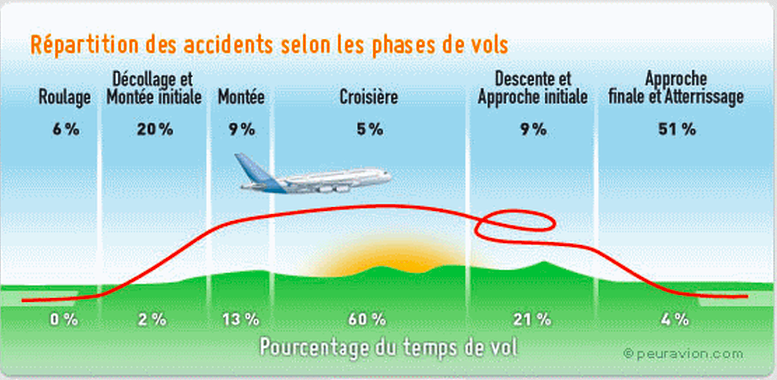
\includegraphics[width=270px]{./crash_avion.png}
 \caption{Statistiques des accidents d'avion en fonction des phases de vol (source peuravion.com)}\label{fig:accidents}
\end{figure}

\begin{enumerate}
 \item (1 point) Indiquer la probabilit\'e qu'un avion de ligne en phase de vol se trouve en phase d'atterrissage. %% 0.5 pts
 \ifcorrection
  \textcolor{red}{On note pour la suite: $T=\{\text{phase d'aTterrissage}\}$ \\
  Selon la Fig.1 on a: $P(T) = 4\% = 0,04$ }
 \fi
 \item (1 point) Indiquer la probabilit\'e qu'un avion accident\'e se soit trouv\'e en phase de croisi\`ere au moment de l'accident . %% 0.5 pts
  \ifcorrection
  \textcolor{red}{ On note $A=\{\text{L'avion a un Accident}\}$ et $C=\{\text{vol de Croisiere}\}$\\
  Selon la Fig.1 on a: $P(C|A) = 5\% = 0,05$  } % $A_{30}^7 = \frac{26!}{19!} = 20 \times 21 \times ... \times 26 = 3~315~312~000 
 \fi
 \item (3 points) Sachant que la probabilit\'e d'avoir un accident d'avion est de 1 sur 12 millions, calculer la probabilit\'e
 d'avoir un accident si on sait que l'avion se trouve en phase d'atterrissage.
 \ifcorrection
  \textcolor{red}{~\\D'apr\`es le theoreme de Bayes, on a:\\
   $P(A|T) = \frac{P(T|A) P(A)}{P(T)} $.\\
  L'\'enonc\'e nous donne $P(A)= \frac{1}{12 \times 10^6}$, $P(T|A) = 0,51$ qui conduit \`a:\\
  $P(A|T) = \frac{0,51 \frac{1}{12 \times 10^6}}{0,04} \approx 1,0625\times 10^{-6}$ 
 }
 \fi
 %\item (2 point) \`A partir du r\'esultat obtenu \`a la question pr\'ec\'edent indiquer par quel facteur multiplicatif la probabilit\'e d'avoir un accident d'avion
  %augmente ou diminue quand on sait que l'avion se trouve en phase d'atterrissage. %R\'epondre \`a la m\^eme question en consid\'erant cette fois la phase de d\'ecollage.
  \ifcorrection
   \textcolor{red}{
  Le facteur multiplicatif d'avoir un accident d'avion quand un avion est en phase d'atterrissage vaut:
   $a_T = \frac{P(A|T)}{P(A)} = \frac{P(T|A)}{P(T)} = \frac{0,51}{0,04} \approx 12,75$.\\
   %
   Pour la phase de d\'ecollage: (on note $D=\{Decollage \}$)\\
  on a $P(A|D) = \frac{P(D|A) P(A)}{P(D)} = \frac{0,2 \frac{1}{12 \times 10^6}}{0,02}$\\
   et donc le facteur multiplicatif d'avoir un accident en phase de d\'ecollage vaut :\\
   $a_D = \frac{P(A|D)}{P(A)} = \frac{P(D|A)}{P(D)} = \frac{0,2}{0,02} = 10$
%  L'\'enonc\'e nous donne $P(A)= \frac{1}{12 \times 10^6}$, $P(T|A) = 0,51$ qui conduit \`a:\\
%  $P(A|T) = \frac{0,51 \frac{1}{12 \times 10^6}}{0,04} \approx 1,0625\times 10^{-6}$ % $A_{30}^7 = \frac{26!}{19!} = 20 \times 21 \times ... \times 26 = 3~315~312~000 
  }
  \fi
\end{enumerate}

%(6 points)
% \exost  Un commer\c{c}ant propose les services suivants: service-A: 40 euros, service-B: 110 euros et 
% service-C: 70 euros. On donne la probabilit\'e (en utilisant la notation $A=\{"\text{choisir le service A}\}$, resp. B et C) 
% qu'un client choisisse une prestation au cours d'une visite: $P(A)=30\%$, $P(B)=10\%$ et $P(C)=20\%$
% ainsi que les probabilit\'es conjointes suivantes: $P(A\cap B) = 8\%$, $P(A\cap C) = 15\%$ et $P(B\cap C) = 3\%$
% 
% \begin{enumerate}
%  \item (1 point) Sachant qu'un client peut demander au maximum 2 services diff\'erents simultan\'ement ou repartir sans achat. 
%  Calculer $\text{card}(\Omega)$, c'est-\`a-dire le nombre distinct de prestations pouvant \^etre demand\'ees par un m\^eme client au cours d'une visite. Vous indiquerez
%  la configuration de d\'enombrement qui s'applique ainsi que la formule de calcul correspondante.
%  \ifcorrection
%  \textcolor{red}{On consid\`ere la somme des combinaisons (tirage non ordonn\'e, sans remise) obtenues par le tirage de $k=0$, $k=1$ et $k=2$ \'el\'ements choisis parmi $n=3$.
%  $N = \sum_{k=0}^2 C_n^k = 1 + 3 + 3 = 7$.}
%  \fi
%  \item (2 points) D\'efinir la variable al\'eatoire $X$ en indiquant la probabilit\'e de chaque \'ev\'enement de $\Omega$
%  qui donne le montant d'une facture (en euros) en fonction des prestations demand\'ees par un client.
%   \ifcorrection
%  \textcolor{red}{
%  $X$ est la fonction $\Omega \rightarrow X(\Omega)$ qui associe \`a chaque \'ev\'enement de $\Omega$ une valeur $x$.\\
%   On note $A,B,C$ les \'ev\'enements associ\'es au tirage du service correspondant permettant de noter les \'ev\'enements suivants associ\'es \`a une valeur distincte $x$ prise par la va $X$:\\
%   \begin{tabular}{|l|l|l|}
%   \hline
%     $\Omega$ 			& $x$	& probabilit\'e	\\
%     \hline
%      \{``aucun service''\}    	& 0	&  0,14 (reste) \\
%      \hline
%      A				& 40	&  0,3 \\
%      \hline 
%      B				& 110	&  0,1 \\
%      \hline
%      C				& 70	& 0,2  \\
%      \hline
%      AB				& 150	& 0,08 \\
%      \hline
%      AC				& 110	& 0,15 \\
%      \hline
%      BC				& 180   & 0,03 \\
%    \hline
%   \end{tabular}
%   ~\\
%   On a donc $\Omega = \{ \{``aucun service''\}, A,B,C,AB,AC,BC \}$ et $X(\Omega) = \{0,40,70,110,150,180\}$.}
%  \fi 
%  \item (2 points)%Sachant que le choix d'une prestation par un client est ind\'ependant de ses choix pr\'ec\'edents,
%  Donner la loi de probabilit\'e de $X$ not\'ee $p_X$ ainsi que sa fonction de r\'epartition $F_X$.
%   \ifcorrection
%  \textcolor{red}{~\\
%  On classe par ordre croissant les valeurs distinctes prises par $X$ et on calcule leurs probabilit\'es en additionnant les probabilit\'es des \'ev\'enements de $\Omega$ correspondants:\\
%   \begin{tabular}{|l|l|l|l|l|l|l|}
%   \hline
%     $x$ 	& 0	& 40	& 70	& 110 	& 150  	& 180 \\
%     \hline
%      $p_X(x)$    	& 0,14	& 0,3	& 0,2	& 0,25 	& 0,08 	& 0,03\\
%      \hline
%      $F_X(x)$	& 0,14  & 0,44	& 0,64	& 0,89	& 0,97	& 1\\
%    \hline
%   \end{tabular}}
%  \fi 
%  \item (1 point) Calculer l'esp\'erance de $X$ not\'ee $E[X]$. % = \sum_x x~P(X=x)$
%    \ifcorrection
%  \textcolor{red}{~\\
%    $E[X] =0 \times 0,14 + 0,3 \times 40 + 70 \times 0,2 + 110 \times 0,25 + 150 \times 0,08 + 180 \times 0,03 = 70,9 $}
%  \fi 
% \end{enumerate}




%Une usine fabriquant des puces informatiques produit une pi\`ece d\'efectueuse pour 1000 produites.
% Un syst\`eme innovant propose de d\'etecte 98\% des pi\`eces d\'efectueuses avec un taux de faux positifs
% de 0,03\%. Est-ce que ce syst\`eme est vraiment efficace? Pour vous en assurer, vous calculerez la probabilit\'e
% qu'une pi\`ece soit d\'efectueuse en cas de d\'etection et vous la comparerez \`a un seuil fix\'e \`a 60\%
% 
%  \ifcorrection
%  \textcolor{red}{
%  On note $P = \{\text{Pi\`ece d\'efectueuse}\}$ et $T=\{\text{Test positif}\}$\\
%  On a alors $P(T|D) = 0.98$, $P(T|\bar{D}) = 3\times 10{-4}$ et $P(D) = 10^{-3}$.\\
%  Le th\'eor\`eme des probabilit\'e totales permet de calculer:
%  $P(T) = P(T|D)P(D) + P(T|\bar{D})P(\bar{D}) = 0,98 \times 10^{-3} + 3\times 10{-4} \times (1-10^{-3}) = 1,3 \times 10^{-3}$.\\
%  Le th\'eor\`eme de Bayes nous permet d'\'ecrire: 
%  $P(D|T) = \frac{P(T|D)P(D)}{P(T)} = \frac{0,98 \times 10^{-3}}{1,3 \times 10^{-3}} \approx 0,7538$\\
%  On en d\'eduit que le syst\`eme de d\'etection est bien efficace!}
%  \fi
%  
% \exost (6 points) On consid\`ere un jeu consistant \`a deviner une combinaisons de 5 nombres
% compris entre 0 et 9, tir\'es al\'eatoirement et sans remise. Le jeu dispose des r\`egles suivantes:
% \begin{itemize}
%  \item On paye 5 euros pour avoir le droit de jouer
%  \item On gagne 6 euros si 3 nombres sont corrects parmi les 5
%  \item On gagne 100 euros si 4 nombres sont corrects parmi les 5
%  \item On gagne 1000 euros si tous les nombres sont corrects % parmi les 5
%  \item On ne gagne rien dans tous les autres cas
% \end{itemize}
% \begin{enumerate}
%  \item D\'efinir la variable al\'eatoire $X$ qui associe le tirage de 5 nombres au gain (bilan final en euros) obtenu en jouant \`a ce jeu.
%  \item D\'efinir la loi de probabilit\'e de $X$ ainsi que sa fonction de r\'epartition.
%   \ifcorrection
%  \textcolor{red}{
%  On consid\`ere le tirage de k=5 nombres parmi 10 tir\'es sans ordre et sans remise.
%  \begin{tabular}{|l|l|l|l|}
%   \hline
%   $\Omega$ & $X$ & $p_X$									& $F_X$\\
%   \hline
%   $\leq 2$ & -5  & $\frac{252-16}{252} = \frac{236}{252} \approx 0.9365$			& 0.9365\\
%   3	   & 1   & $\frac{C_{5}^3}{C_{10}^3} = \frac{10}{252}\approx 3,97 \times 10^{-2} $	& 0.9762\\
%   4	   & 95  & $\frac{C_{5}^4}{C_{10}^4} = \frac{5}{252} \approx 1,98 \times 10^{-2} $	& 0.9960\\
%   5	   & 995 & $\frac{C_{5}^5}{C_{10}^5} = \frac{1}{252} \approx 4 \times 10^{-3} $		& 1\\
%   \hline
%  \end{tabular}
%  }
%  \fi
% %
%  \item Au bout de combien de tentatives la probabilit\'e de gagner au moins 90 euros est sup\'erieure \`a 90\%.
%    \ifcorrection
%  \textcolor{red}{
%  On note $A=\{ X \geq 90 \}$\\
%  $P(A) = P(X=95) + P(X=995) = \frac{6}{252} \approx 2,38\times 10^{-2}$\\
%  Donc a $P(\bar{A}) = 1-P(A) \approx 0,9762$. 
%  En consid\'erant chaque tirage comme ind\'ependant, la probabilit\'e de ne rien gagner apr\`es $n$ essais est de $P(\bar{A})^n$.\\
%  On cherche donc \`a r\'esoudre l'in\'equation suivante:
%  \begin{align}
%   1 - P(\bar{A})^n &> 0,9\\
%   0,1 &> P(\bar{A})^n \\
%   \log(0,1) &> n \log(P(\bar{A}))\\
%   n &> \frac{\log(0,1)}{\log(P(\bar{A}))} \approx 95,5914
%  \end{align}\\
%  On d\'eduit qu'il faut au moin 96 tentatives pour avoir 90\% de chance de gagner plus de 90 euros.
%  }
%  \fi
% \end{enumerate}


% P(T|D) = 0,999   P(T|\bar{D}) = 0,003  P(D) = 10^{-3}
% 
% P(T) = P(T|D) P(D) + P(T|\bar{D}) (1-P(\bar{D})) = 
% 
% P(D|T) = P(T|D) P(D) / P(T)


\end{document}

% End Of File

